%%%%%%%%%%%%%%%%%%%%%%%%%%%%%%%%%%%%%%%%%%%%%%%%%%%%%%%%%%%%%%%%%%%%%%%%%%%%%%%%
%2345678901234567890123456789012345678901234567890123456789012345678901234567890
%        1         2         3         4         5         6         7         8

\documentclass[letterpaper, 10 pt, conference]{ieeeconf}  % Comment this line out
                                                          % if you need a4paper
%\documentclass[a4paper, 10pt, conference]{ieeeconf}      % Use this line for a4
                                                          % paper

\IEEEoverridecommandlockouts                              % This command is only
                                                          % needed if you want to
                                                          % use the \thanks command
\overrideIEEEmargins
% See the \addtolength command later in the file to balance the column lengths
% on the last page of the document

\usepackage{graphicx} %package to manage images
\graphicspath{ {images/} }

% The following packages can be found on http:\\www.ctan.org
%\usepackage{graphics} % for pdf, bitmapped graphics files
%\usepackage{epsfig} % for postscript graphics files
%\usepackage{mathptmx} % assumes new font selection scheme installed
%\usepackage{times} % assumes new font selection scheme installed
%\usepackage{amsmath} % assumes amsmath package installed
%\usepackage{amssymb}  % assumes amsmath package installed

\title{\LARGE \bf
Latido del coraz\'on de un gato*
}

%\author{ \parbox{3 in}{\centering Huibert Kwakernaak*
%         \thanks{*Use the $\backslash$thanks command to put information here}\\
%         Faculty of Electrical Engineering, Mathematics and Computer Science\\
%         University of Twente\\
%         7500 AE Enschede, The Netherlands\\
%         {\tt\small h.kwakernaak@autsubmit.com}}
%         \hspace*{ 0.5 in}
%         \parbox{3 in}{ \centering Pradeep Misra**
%         \thanks{**The footnote marks may be inserted manually}\\
%        Department of Electrical Engineering \\
%         Wright State University\\
%         Dayton, OH 45435, USA\\
%         {\tt\small pmisra@cs.wright.edu}}
%}

\author{Leidy Marcela Aldana Burgos$^{1}$ %and Pradeep Misra$^{2}$% <-this % stops a space
%\thanks{*This work was not supported by any organization}% <-this % stops a space
\thanks{$^{1}$Estudiante Ingenier\'ia de Sistemas,
        Universidad Distrital Francisco Jos\'e de Caldas.
        {\tt\small lmaldanab@correo.udistrital.edu.co}}%
%\thanks{$^{2}$P. Misra is with the Department of Electrical Engineering, Wright State University,
 %       Dayton, OH 45435, USA
  %      {\tt\small p.misra at ieee.org}}%
}


\begin{document}



\maketitle
\thispagestyle{empty}
\pagestyle{empty}


%%%%%%%%%%%%%%%%%%%%%%%%%%%%%%%%%%%%%%%%%%%%%%%%%%%%%%%%%%%%%%%%%%%%%%%%%%%%%%%%
\begin{abstract}

This project will develop a device that obtains the heartbeat of a cat, with the aim of helping veterinary medicine to give accurate reports in cases of heart failure, which is a problem that can affect cats.\\

The open-source platform that will be used is Arduino since there is a sensor that complies with this functionality, detecting heartbeats, in addition, it can be programmed using an IDE and its own programming language.

\end{abstract}


%%%%%%%%%%%%%%%%%%%%%%%%%%%%%%%%%%%%%%%%%%%%%%%%%%%%%%%%%%%%%%%%%%%%%%%%%%%%%%%%
\section{INTRODUCCI\'ON}

Los gatos tienen diferentes tipos de problemas cardiacos, los cuales, pueden ser tratados si se diagnostican a tiempo, con el objetivo de lograr un diagn\'ostico oportuno se desarrollar\'a un dispositivo que detectar\'a las anormalidades del latido del coraz\'on del felino, enviando r\'apidamente un mensaje al responsable del mismo, y si la anormalidad persiste se enviar\'a un reporte al veterinario.
\\

Este dispositivo requerir\'a dedicar tiempo al aprendizaje de Arduino y la implementaci\'on de uno de sus sensores, la propuesta de la utilizaci\'on de esta plataforma libre se basa en la idea de \textit{Vimos, Sacoto, Morales 2016}, la cual postula \textit{"La simplicidad en el uso de estos dispositivos ha provocado que el n\'umero de proyectos que hacen uso de este tipo de hardware se incremente cada d\'ia."} (ver referencia \cite{c1})

\section{JUSTIFICACI\'ON}

Este proyecto generar\'a documentaci\'on libre, dado que el conocimiento adquirido ser\'a publicado a trav\'es de tres (3) art\'iculos para que la comunidad pueda acceder; adem\'as, se necesitar\'a tener (o adquirir) un buen conocimiento en diferentes \'areas como Internet de las cosas, Arduino, manejo de sensores, entre otros.

\section{OBJETIVOS}

\subsection{OBJETIVO GENERAL}

Desarrollar un dispositivo que obtenga el latido del coraz\'on de un gato, para generar un reporte y posibles alertas implementando el sensor KY-039 de Arduino.

\subsection{OBJETIVOS ESPEC\'IFICOS}

\begin{itemize}
    \item Aprender a utilizar la plataforma Arduino
    \item Implementar el sensor KY-039 como detector del latido del coraz\'on en relaci\'on a posibles fallos
    \item Evaluar si el dispositivo lograr\'a los objetivos propuestos en el proyecto
    \item Convalidar el correcto funcionamiento del Arduino con su sensor
    \item Desarrollar una aplicaci\'on para visualizar los latidos del coraz\'on del gato
    \item Generar un paso de mensajes entre el Arduino y la aplicaci\'on 
    \item Crear un reporte de los datos registrados por el dispositivo
\end{itemize}

\section{DESCRIPCI\'ON DE RECURSOS}

\begin{itemize}

    \item 
        \textbf{Recurso:} Arduino\\
        \textbf{Justificaci\'on:} Plataforma open-source para controlar y hacer uso del sensor que toma los latidos\\
        
    \item 
        \textbf{Recurso:} Sensor KY-039\\
        \textbf{Justificaci\'on:} M\'odulo de Arduino que detecta el latido del coraz\'on\\
        
    \item 
        \textbf{Recurso:} IDE\\
        \textbf{Justificaci\'on:} Integrated Development Environment para Arduino\\
        
    \item 
        \textbf{Recurso:} Overleaf\\
        \textbf{Justificaci\'on:} Editor de LaTeX en l\'inea para realizar la documentaci\'on del proyecto\\
    
    \item 
        \textbf{Recurso:} Marvel\\
        \textbf{Justificaci\'on:} Editor para creaci\'on de prototipos\\
        % https://marvelapp.com/
        
     \item 
        \textbf{Recurso:} Postgres\\
        \textbf{Justificaci\'on:} Sistema manejador de Base de datos\\
        
\end{itemize}



\section{TRABAJOS RELACIONADOS}
%using \TeX. If you are using multiple \TeX\ files you must make sure that the ``MAIN`` source file is called root.tex - this is particularly important if your conference is using PaperPlaza's built in \TeX\ to PDF conversion tool.

\subsection{Heart Rate Monitoring System using IR base Sensor \& Arduino Uno  \cite{c7}}

\textit{Prajakta A. Pawar}, el autor de este art\'iculo parte de la necesidad de un monitoreo constante del paciente humano, as\'i, como soluci\'on plantea un sistema que monitorea el latido del coraz\'on humano para enviarlo al doctor utilizando Arduino y el m\'odulo GSM.\\

Este proyecto, comparte la necesidad de este proyecto pero orientado a animales; por lo cual servir\'a como gu\'ia en la estructuraci\'on, es decir, por si alguna idea puede complementarse.\\

Adem\'as, en contraste al mismo, la documentaci\'on de este proyecto referenciar\'a el sensor no s\'olo por su utilidad, sino por la referencia en el mercado contemplando una posible replicaci\'on del mismo.

% https://ieeexplore-ieee-org.bdigital.udistrital.edu.co/stamp/stamp.jsp?tp=&arnumber=7057005

\subsection{Definici\'on conceptual de Arquitectura: Implementaci\'on de una red de sensores usando dispositivos Arduino y aplicaciones multiplataforma mediante el est\'andar OPC UA. \cite{c1}}

En este art\'iculo el autor plantea una arquitectura OPC en relaci\'on a unos sensores de Arduino y a un servidor OPC. Despu\'es se hace enf\'asis en garantizar la sincronizaci\'on de los datos enviados desde diferentes puertas de enlace (Gateways OPC), para lo cual se requiere que cada elemento est\'e sincronizado con un servicio de Network Time Protocol \textit{NTP}. Finalmente, se muestran algunos resultados del servidor de an\'alisis de datos.\\

Para el proyecto planteado, se utilizar\'a el servicio de Network Time Protocol \textit{NTP}; de acuerdo a lo le\'ido acerca de este caso, la implementaci\'on de red de sensores.

\begin{figure}
\centering
\label{fig:uno}
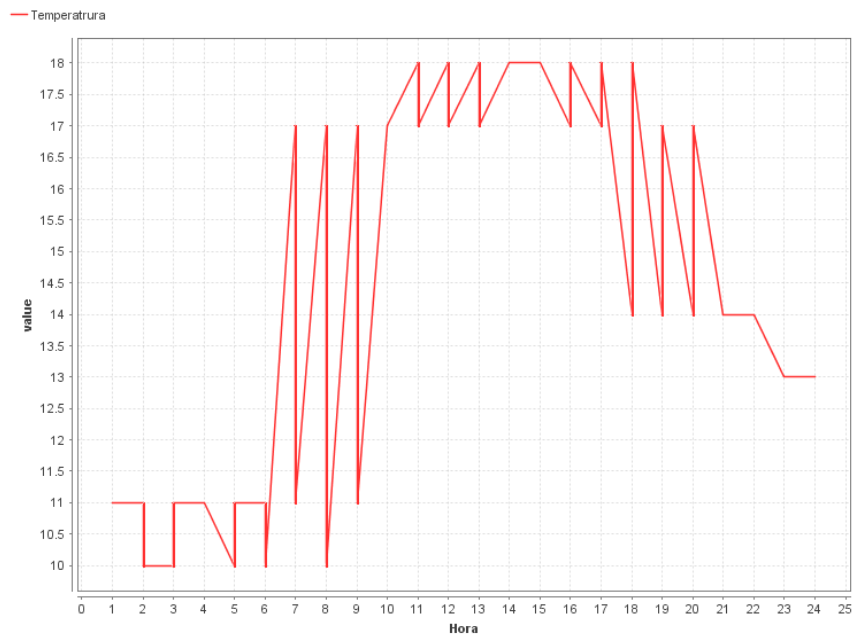
\includegraphics[width=0.45\textwidth]{temperatura.png}
\caption{Figura 5 tomada de \cite{c1}}
\end{figure}

% https://ieeexplore-ieee-org.bdigital.udistrital.edu.co/stamp/stamp.jsp?tp=&arnumber=7778476&tag=1

\subsection{Heart rate and arrhythmia frequency of normal cats compared to cats with asymptomatic hypertrophic cardiomyopathy. \cite{c2}}

Este art\'iculo muestra un estudio realizado a diferentes gatos, con el objetivo de comparar la frecuencia y complejidad de la arritmia de 24 horas en gatos con HCM asintom\'atica y gato normal.\\

Adem\'as, proporciona para el proyecto la justificaci\'on de existencia de enfermedades del coraz\'on en gatos.
% https://ac-els-cdn-com.bdigital.udistrital.edu.co/S1760273414000642/1-s2.0-S1760273414000642-main.pdf?_tid=e27ff1f5-a272-4aac-9c42-0b2334c2ca72&acdnat=1536618156_472cfb81d9484ae2b170e7f0e3e824f8

\subsection{Diagnostic accuracy of plasma atrial natriuretic peptide concentrations in cats with and without cardiomyopathies. \cite{c3}}

Este art\'iculo muestra un estudio que hace uso de una ecocardiograf\'ia para determinar gatos enfermos, subdivididos en gatos asintom\'aticos sin dilataci\'on auricular izquierda (DAI), gatos asintom\'aticos con DAI y gatos con insuficiencia card\'iaca.\\ % https://ac-els-cdn-com.bdigital.udistrital.edu.co/S1760273417302047/1-s2.0-S1760273417302047-main.pdf?_tid=195ad301-2acc-4ebf-8365-2755063e3560&acdnat=1536618934_4f51babde492065888087b88ebf91787

Al igual que la cita anterior, este art\'iculo proporciona bases en conocimiento de las diferentes enfermedades en gatos a nivel del sistema cardiovascular.

\subsection{e-Health: Biomedical instrumentation with Arduino \cite{c5}}

Este art\'iculo describe  el desarrollo de actividades de laboratorio para la introducci\'on al sistema biom\'edico utilizando Arduino, as\'i como algunas experiencias y resultados obtenidos de ellas.\\

As\'i, relaciona la tecnolog\'ia arduino con las necesidades m\'edicas a nivel humano.

% https://ac-els-cdn-com.bdigital.udistrital.edu.co/S2405896317323339/1-s2.0-S2405896317323339-main.pdf?_tid=330640b6-9a7b-4fb4-a494-634c267aa56f&acdnat=1536774498_fd12624c4efcb28253fda8233328c3d9

\subsection{Taking Arduino to the Internet of Things: The ASIP programming model \cite{c6}}

En este art\'iculo se da a conocer el modelo Servicio de Interfaz de Programaci\'on Arduino (ASPI), con su implementaci\'on, su respectivo modelo de clases.

% https://ac-els-cdn-com.bdigital.udistrital.edu.co/S0140366416300743/1-s2.0-S0140366416300743-main.pdf?_tid=471d00b0-f5ab-4dc7-9198-0cd5f9a0df18&acdnat=1536774542_24e1c944d490200cbb0757eaa3a29b7f




\section{METODOLOG\'IA}

Este proyecto se orienta a la construcci\'on de un sistema complejo, que puede incrementar sus requerimientos con el paso del tiempo, por esto la metodolog\'ia empleada para el desarrollo del proyecto implementa un modelo de proceso evolutivo, desarrollando as\'i versiones cada vez m\'as completas del Software.\\



\subsection{Prototipos}

Este proyecto tiene una determinada necesidad, sin embargo, no se han determinado los detalles espec\'ificos. As\'i, la implementaci\'on de un modelo de prototipos facilita la comprensi\'on del sistema, teniendo en cuenta que la aplicaci\'on del mismo se hace con un enfoque evolutivo.\\

Adem\'as, se resaltan las dificultades que podr\'ian tenerse:

\begin{itemize}
    \item Las posibles elecciones inadecuadas que puedan tomarse con el objetivo de lograr funcionalidad en el menor tiempo posible.
    \item Rehacer el producto al final, basados en el prototipo realizado durante el desarrollo.
\end{itemize}


%\begin{table}[h]
%\caption{An Example of a Table}
%\label{table_example}
%\begin{center}
%\begin{tabular}{|c||c|}
%\hline
%One & Two\\
%\hline
%Three & Four\\
%\hline
%\end{tabular}
%\end{center}
%\end{table}

\subsection{Metodolog\'ia de trabajo}

Desde la perspectiva de la Ingenier\'ia de Software, se han planteado los siguientes casos de uso \ref{fig:Casosdeuso}:

\begin{figure}
\centering
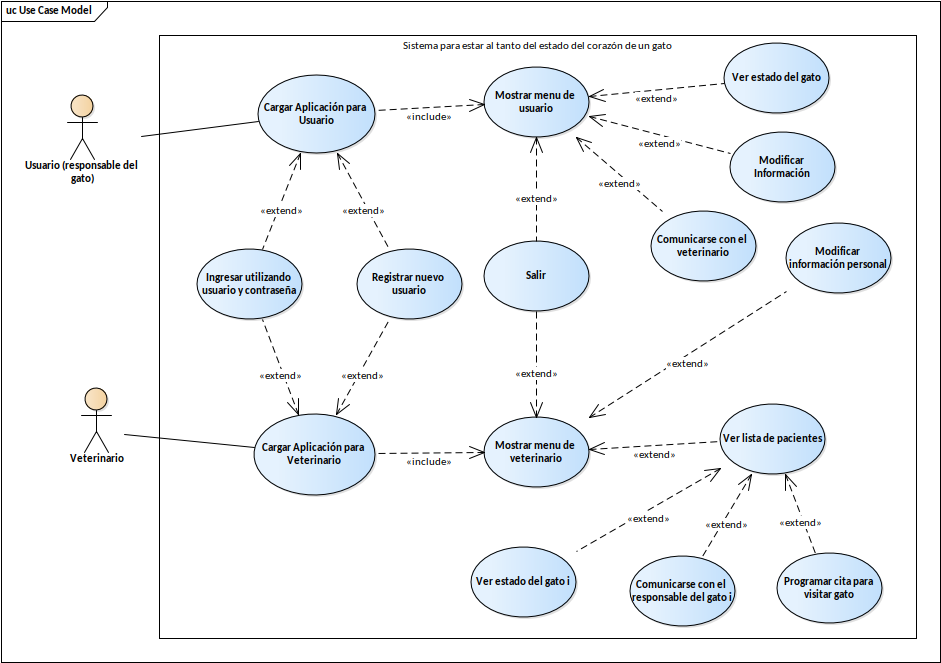
\includegraphics[width=0.5\textwidth]{casousoheartcat.png}
\caption{Primera versi\'on Casos de uso para la aplicaci\'on}
\label{fig:Casosdeuso}
\end{figure}

Los cuales requieren el manejo de una base de datos, la cual se plantea en una primera versi\'on en la figura \ref{fig:entidades}:

\begin{figure}
\centering
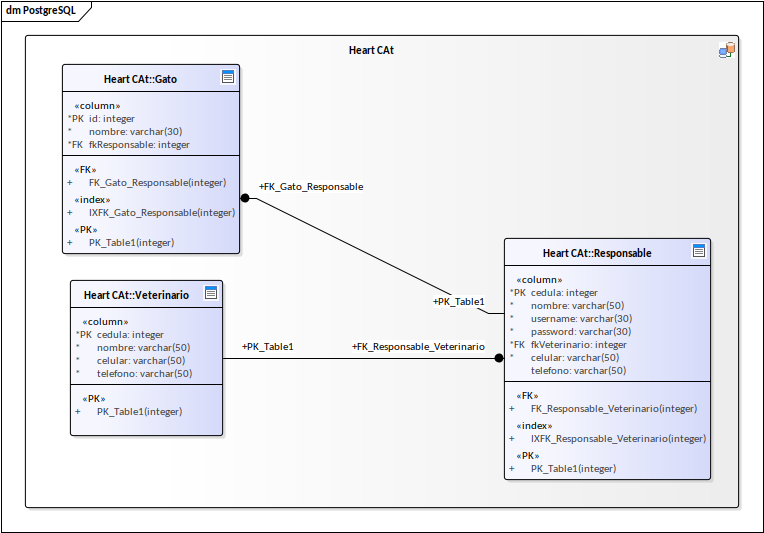
\includegraphics[width=0.5\textwidth]{bdvunoheartcat.png}
\caption{Primera versi\'on tabla entidad relaci\'on para estructuraci\'on de la base de datos}
\label{fig:entidades}
\end{figure}


   
\section{DISE\~NO}

Utilizando la herramienta \textit{Marvel}, se ha creado el primer prototipo de la apliaci\'on con la que interactuar\'a el usuario:

\begin{figure}
\centering
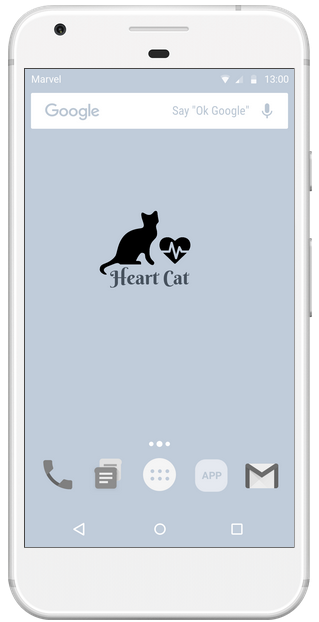
\includegraphics[width=0.2\textwidth]{hc1.png}
\caption{Logo aplicaci\'on vista desde un sistema Android}
\label{fig:home}
\end{figure}

El usuario, una vez accede a la aplicaci\'on se encontrar\'a con ese sistema de logueo \ref{fig:login}, el cual le presenta dos opciones, ingresar con una cuenta existente o crear una nueva. As\'i, se presenta la necesidad de manejar una base de datos.\\

\begin{figure}
\centering
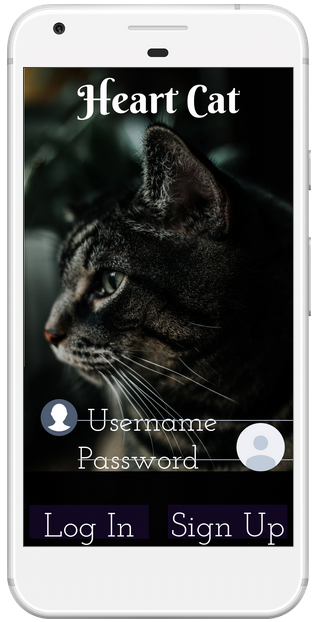
\includegraphics[width=0.2\textwidth]{hc2.png}
\label{fig:login}
\caption{Vista para iniciar sesi\'on}
\end{figure}

En la imagen \ref{fig:signup} podemos ver el primer prototipo de registros para usuarios sin una cuenta.\\

\begin{figure}
\centering
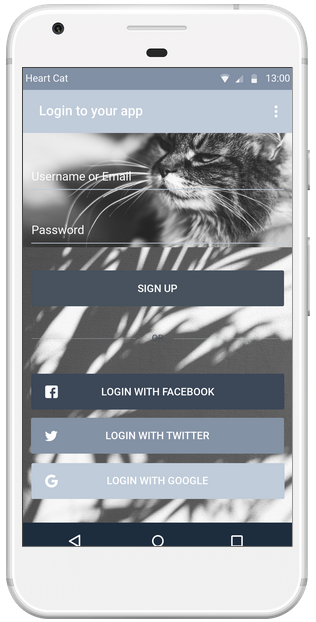
\includegraphics[width=0.2\textwidth]{hc3.PNG}
\label{fig:signup}
\caption{Registro de nuevos usuarios}
\end{figure}

Una vez el usuario accede con su usuario y contrase\~na, puede ver el men\'u principal \ref{fig:menu}, el cual le permitir\'a llamar o enviar un mensaje de texto al veterinario, modificar la informaci\'on actual, ver el estado o salir.\\

\begin{figure}
\centering
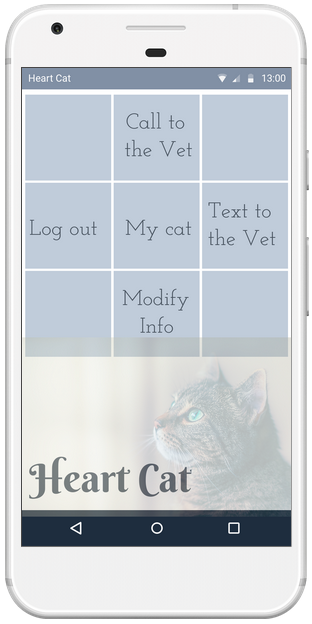
\includegraphics[width=0.2\textwidth]{hc4.PNG}
\label{fig:menu}
\caption{Menu principal para el responsable del gato}
\end{figure}

\begin{figure}
\centering
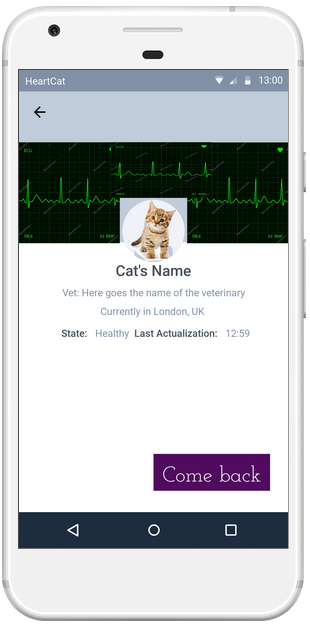
\includegraphics[width=0.2\textwidth]{HC5.PNG}
\label{fig:viewingHeart}
\caption{Visualizaci\'on del estado de salud}
\end{figure}

\section{IMPLEMENTACI\'ON}

Se realiz\'o el montaje f\'isico entre el arduino, el sensor, y la conexi\'on a un PC para la toma de datos utilizando el programa \textit{Arduino}.

\begin{figure}
\centering
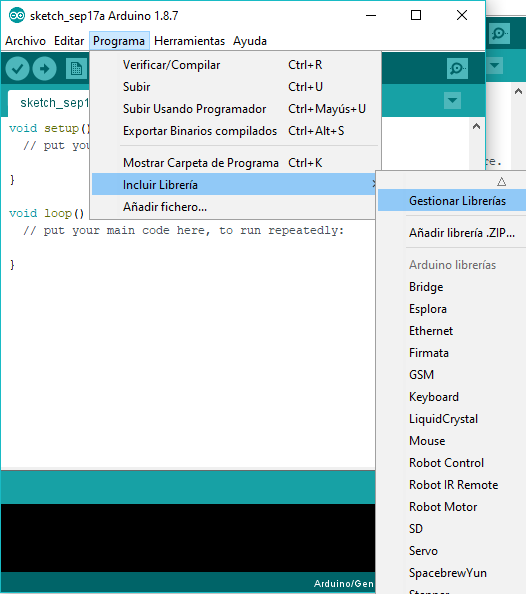
\includegraphics[width=0.5\textwidth]{includeLibrary.png}
\label{fig:library}
\caption{Incluyendo la librer\'ia para graficar}
\end{figure}

Para la graficaci\'on de los datos recibidos, se ha dise\~nado el siguiente c\'odigo \ref{fig:code}:

\begin{figure}
\centering
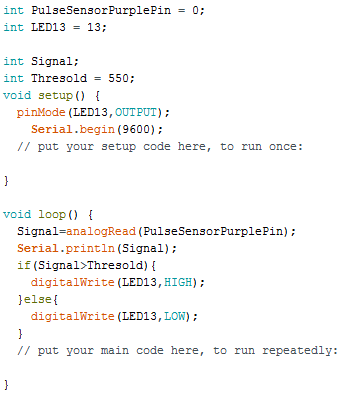
\includegraphics[width=0.35\textwidth]{codeArduino.png}
\label{fig:code}
\caption{C\'odigo utilizado para recibir y graficar los pulsos}
\end{figure}

Gracias a lo cual, se tomaron datos en un ser humano:
% AÑADIR IMAGEN MANO

Generando la siguiente gr\'afica \ref{fig:senal}:
 
\begin{figure}
\centering
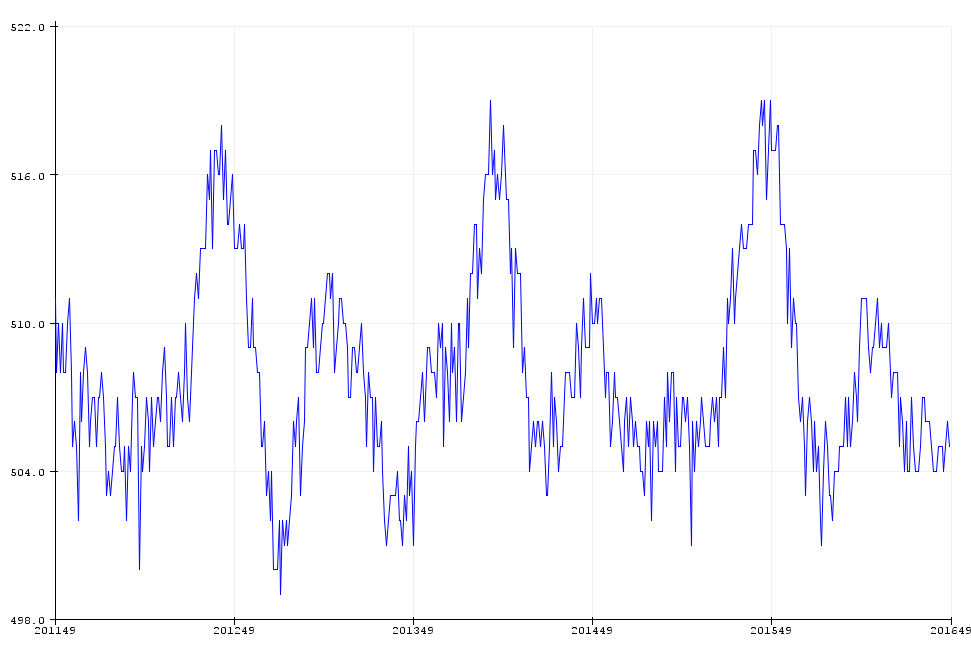
\includegraphics[width=0.4\textwidth]{senal.png}
\label{fig:senal}
\caption{Gr\'afica de la se\~nal}
\end{figure}

La cual corresponde con los principales intervalos del latido humano:

\begin{figure}
\centering
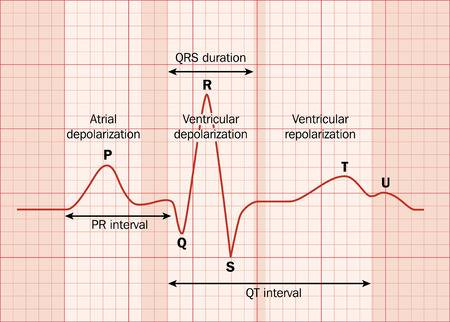
\includegraphics[width=0.4\textwidth]{ecg.jpg}
\label{fig:intervalo}
\caption{Intervalos del latido del coraz\'on humano}
\end{figure}

\section{CONCLUSIONES}

De acuerdo a los trabajos relacionados, se puede observar que no hay muchos estudios realizados que relacionen las dos \'areas; el \'area veterinaria se ha centrado en estudiar las enfermedades y el \'area de ingener\'ia se ha centrado en la aplicaci\'on de las ciencias b\'asicas para la soluci\'on de problemas.\\

As\'i es viable un estudio que implica ambas ciencias, el cual ser\'a desarrollado utilizando la metodolog\'ia de software basada en prototipos, la cual bajo el enfoque evolutivo permitir\'a tener un desarrollo r\'apido.

\addtolength{\textheight}{-12cm}   % This command serves to balance the column lengths
                                  % on the last page of the document manually. It shortens
                                  % the textheight of the last page by a suitable amount.
                                  % This command does not take effect until the next page
                                  % so it should come on the page before the last. Make
                                  % sure that you do not shorten the textheight too much.

%%%%%%%%%%%%%%%%%%%%%%%%%%%%%%%%%%%%%%%%%%%%%%%%%%%%%%%%%%%%%%%%%%%%%%%%%%%%%%%%



%%%%%%%%%%%%%%%%%%%%%%%%%%%%%%%%%%%%%%%%%%%%%%%%%%%%%%%%%%%%%%%%%%%%%%%%%%%%%%%%



%%%%%%%%%%%%%%%%%%%%%%%%%%%%%%%%%%%%%%%%%%%%%%%%%%%%%%%%%%%%%%%%%%%%%%%%%%%%%%%%
%\section*{APPENDIX}

%Appendixes should appear before the acknowledgment.

%\section*{ACKNOWLEDGMENT}




%%%%%%%%%%%%%%%%%%%%%%%%%%%%%%%%%%%%%%%%%%%%%%%%%%%%%%%%%%%%%%%%%%%%%%%%%%%%%%%%




\begin{thebibliography}{99}

\bibitem{c1} V. Vimos, E. Sacoto, D.X. Morales, \textit{Conceptual Architecture Definition: Implementation of a Network Sensor Using Arduino Devices and Multiplatform Applications through OPC UA.}.\\

\bibitem{c2} Bethany L. Jackson, DVM*, Linda B. Lehmkuhl, DVM, MS ,Darcy B. Adin, DVM. \textit{Heart rate and arrhythmia frequency of normal cats compared to cats withasymptomatic hypertrophic cardiomyopathy}. Journal of Veterinary Cardiology (2014). \\ 

\bibitem{c3} Y. Heishima, DVMa,b, Y. Hori, DVM, PhDa,*, K. Nakamura,DVM, PhDc, Y. Yamashita, DVMd, N. Isayama, DVM, PhDe,N. Kanno, DVM, PhDf, M. Katagi, DVMg, H. Onodera, DVMh,S. Yamano, DVMi, Y. Aramaki, DVM, PhD. \textit{Diagnostic accuracy of plasma atrial natriuretic peptide concentrations in cats with and without cardiomyopathies}.  (2018) Journal of Veterinary Cardiology. \\

\bibitem{c4} Pressman S. Roger, \textit{Ingenier\'ia del software, un enfoque pr\'actico.} S\'eptima edici\'on. Editorial The Mc Graw-Hill. M\'exico. Cap\'itulo 2. Modelos del Proceso. ISBN: 978-607-15-0314-5.\\

\bibitem{c5} Puente, S.T.* Úbeda, A.* Torres, F. \textit{e-Health: Biomedical instrumentation with Arduino}. Physics, Systems Engineering and Signal Theory Department, University of Alicante, Spain (2017).\\

\bibitem{c6} Gianluca Barbon, Michael Margolis, Filippo Palumbo, FrancoRaimondi, Nick Weldin, \textit{Taking Arduino to the Internet of Things: The ASIP programming model}\\

\bibitem{c7} Prajakta A. Pawar, \textit{Heart Rate Monitoring System using IR base Sensor \& Arduino Uno.} Department of Instrumentation Engineering Vishwakarma  Institute of  Technology. India.\\

\bibitem{c8} P\'agina oficial sensor de pulso Arduino, consultada el lunes 17 de Septiembre de 2018, disponible en:\\ https://pulsesensor.com/pages/two-or-more-pulse-sensors


\end{thebibliography}




\end{document}
